\section{Introduction to Security on Commodity Systems}

\textbf{Several Things have to be protected:}
\begin{itemize}
    \item[-]OS: manages and shares hardware resources between applications.
    \item[-]Hardware resources: CPU, memory, peripherals
    \item[-]Application: code, data (volatile, persistent)
\end{itemize}{}

\subsection{Application Security}
\textbf{Three important properties: }
\begin{itemize}
    \item[1.]\textbf{Launch-time integrity: }pristine/correct application was started or loaded. (Hash verification of initial code, data)
    \item[2.]\textbf{Run-time isolation: }no interference from malicious software, peripherals. (Prevention of unauthorized modification of code and data, and prevention of run-time attacks e.g. code injection)
    \item[3.]\textbf{Secure persistent storage: } Confidentiality, integrity protection of persistent data.
\end{itemize}{}

\subsubsection{Trusted OS-based Solution} 

\paragraph{What type of hardware-support in x86-systems for OS-based application security?}

\paragraph{Three main components: }
\begin{itemize}
    \item[-]\textbf{Processor: }contains one or more CPU's
    \item[-]\textbf{Chipset: }connects the processor to memory(RAM) and peripherals.
    \item[-]\textbf{Peripherals: }connect via various bus-interfaces to the chipset.
\end{itemize}{}

\paragraph{Privilege Rings}
\begin{itemize}
    \item[0.]Kernel
    \item[1.]Device drivers
    \item[2.]Device drivers
    \item[3.]Applications
\end{itemize}

\paragraph{Memory Management Unit (MMU)}
Translates virtual addresses to physical addresses by traversing the appropriate page tables (kernel page table, app1 page table)

\paragraph{Paging-based Security: }Security-relevant data in page table entries.
\begin{itemize}
    \item[-]\textbf{Supervisor bit: }if set this page is accessible only in ring 0 (isolates OS from applications)
    \item[-]\textbf{RW bits: }to distinguish between read-only and writeable pages.
    \item[-]\textbf{Execution disabel (ED) bit: }if set, the page is not executable (prevents run-time code injection)
\end{itemize}

\paragraph{Firewire DMA}
Access to RAM is tightly controlled by the CPU. But this can be circumvented through DMA(Direct Memory Access)\\
$\rightarrow$ allows fast communication speeds between devices.\\
$\rightarrow$ Attacker can use Firewire cable to issue a DMA request to fetch the contents of RAM.
\textbf{Solution: }IOMMU controls the DMA accesses!

\paragraph{Attacks using physical access}
Physical Access Attacks are harder to defend for the OS. E.g remove hard drive and plug it into other system.\\
\\
\textbf{Some broken Solutions: }
\begin{itemize}
    \item[-]BIOS Protection: Prevent booting from external sources (Broken!)
    \item[-]Disk Encryption: The entire disk is encrypted and unlocked providing a secret key (possible to find key & can still wipe the disk)
    \item[-]Disk Encryption 2. Attempt: use password only, decryption key is protected by password (can brute force password)
    \item[-]Disk Encryption 3. Attempt: leverage a secure element Trusted Platform Module (TPM) chip. Use password to encrypt decryption key on TPM.
\end{itemize}

\paragraph{Disk Encryption}
Data on disk is always stored encrypted. User supplies a key/password to the encryption layer. File System is completely unaware. Regardless of the unlocking technique, the encryption key must be kept in memory. Therefore Encryption key can be read even after platform is powered off (cold boot attack).\\
\paragraph{Cold Boot Attack: } Assumption that DRAM loses its content soon as a machine remains without power is wrong.
\textbf{Solutions: }
\begin{itemize}
    \item[-]Erase Key: user needs to type in password often.
    \item[-]Prevent Booting from external media. Does not prevent DRAM component transfers
    \item[-]Physical Protection: components that respond to enclosure opening or low temperatures (expensive)
    \item[-]Avoid placing key in memory (requires architectural changes.
\end{itemize}{}

\paragraph{TPM Support: } lecture 4 slide 39ff

\subsection{Application Security: Trusted Execution Environments}
Secure launch $\rightarrow$ Isolated Execution $\rightarrow$ Secure Persistent Storage

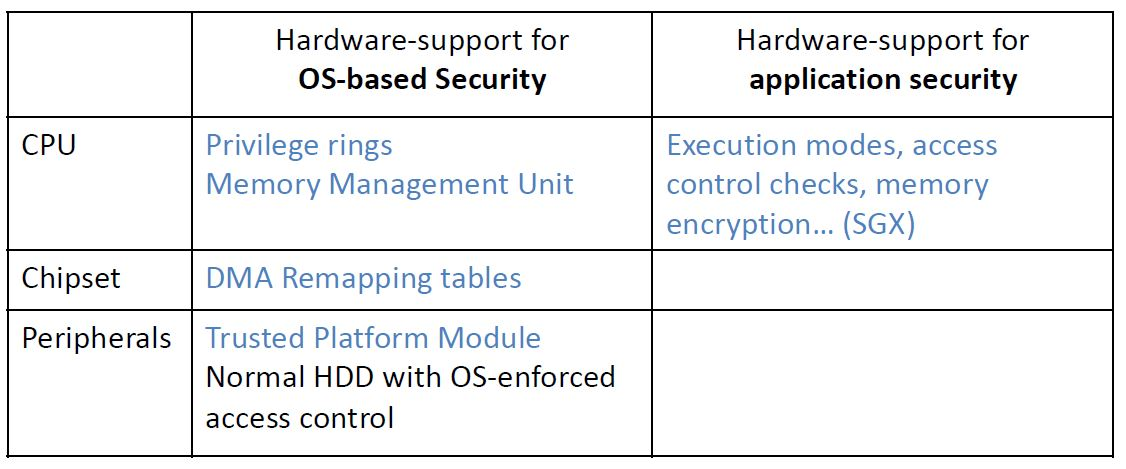
\includegraphics[scale=0.75]{Figures/App-Security.JPG}

\paragraph{Lesson Learned: Trusting OS can make some security functions easier but as the OS is complex its prone to errors.}

\paragraph{ARM TrustZone (a TEE)} Secure virtual processor realized as a special CPU-Mode, managed by a small trusted OS 

\paragraph{Intel SGX (Software Guard Extension) (a TEE)} Untrusted OS manages TEE memory but cannot access it.

\paragraph{Bad USB (Attacks by Untrusted Peripherals)} change a USB device controller to mimic another device class. E.g. Storage device acts as keyboard and opens console.

\paragraph{Case Study: Smartphone Storage Protection}
No TPM! Solution: leverage hardware support in the platform (processor specific keys(ARM TrustZone)). Processor chip has device-specific encryption keys - Extracting such keys not easy risk damaging chip. Use PIN and key to derive storage encryption key. Prevents brute forcing of extracted storage.
\\
\\
How to control PIN attempts? slide 52 lecture 4

\subsection{Intel SGX}
\paragraph{Intel Software Guard Extensions: }Intels new architecture containing new instructions and protecive mechanism in the processor.
$\rightarrow$ Hardening even if you trust the OS.\\
\\
\begin{itemize}
    \item[-]Company app calls the enclave, which then executes and returns.
    \item[-]Enclave memory is encrypted (and integrity protected) at the processor boundary.
\end{itemize}

\paragraph{Sealing: }
\begin{itemize}
    \item[-]Enclave has no direct access to disk or IO/ No access to persistent storage.
    \item[-]No direct access to trusted clock, limited support for counters
    \item[-]Can do sealing: store encrypted confidential data on disk.
    \item[-]When building an enclave, SGX generates a cryptographic log of all the build activities.(MRENCLAVE is a digest of the logs of build process and used as id of an enclave)
    \item[-]Same ID on the same platform can unseal what was previously sealed.
\end{itemize}

\paragraph{Secure communication to/from Enclave:}
Create Enclave Secure Channel....

\paragraph{Remote Attestation: }
During manufacturing 2 keys are burned into the CPU: 
\begin{itemize}
    \item[-]Fused Seal Key is used as Processors secret
    \item[-]Provisioning Key serves as a proof for remote Platform
\end{itemize}

\subsection{DelegaTEE: Brokered Delegation using TEEs}
Reading!!
\paragraph{Properties: }
\begin{itemize}
    \item[-]The Owners credentials remain confidential.
    \item[-]The Owner can restrict access to his account, e.g. in terms of time, duration of access, no. of reads/writes etc.
    \item[-]The system logs the actions of Owners and Delegatees so that post-hoc attribution of their behaviour is possible.
    \item[-]The system minimizes the ability of a service to distinguish between access by the Delegatee and that of the legitimate Owner.
    \item[-]Owner does not have to always be online.
\end{itemize}

